\chapter{Grundlagen}

\section{Google Design Sprint}

Der Google Design Sprint (GDS) ist eine von Jake Knapp bei Google Ventures entwickelte Methodik zur schnellen und effizienten Problemlösung sowie Produktentwicklung, insbesondere für Herausforderungen, die sich aus der dynamischen Natur des Marktes und den sich verändernden Produktanforderungen ergeben. 
Ziel dieser Methode ist es, innerhalb eines Zeitraums von fünf Tagen einen Prototyp zu entwickeln und zu evaluieren. 
Diese Methode bietet den Vorteil, dass nicht auf die Markteinführung gewartet werden muss, um Feedback zu erhalten. Stattdessen können dringende Fragen sofort beantwortet werden \cite[S.98 f.]{Design_Sprint}.

Die fünftägige Methode, wie in Abbildung \ref{GDS} dargestellt, verläuft wie folgt:

\begin{figure}[h]
    \centering
    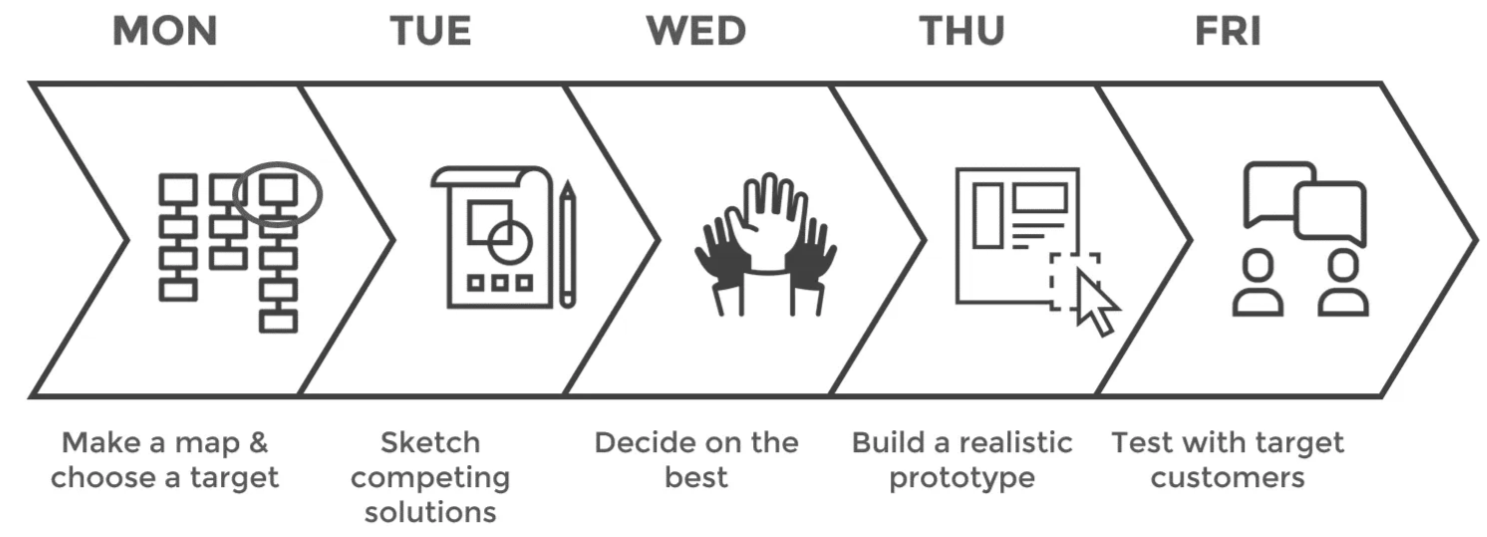
\includegraphics[clip,width=0.75\linewidth]{images/GDS.png}
    \caption[Ablauf eines GDS]{Ablauf eines GDS \cite{GDS_Abbildung}}
    \label{GDS}
\end{figure}

Am ersten Tag geht es darum, das Problem zu verstehen und den Fokus für die Woche festzulegen. Das Team definiert das langfristige Ziel und identifiziert die Herausforderung. 

Am zweiten Tag konzentriert sich das Team auf die Bewältigung bereits bekannter Herausforderungen. Anders als bei herkömmlichen Brainstorming-Sitzungen arbeiten die Teammitglieder einzeln an Lösungsansätzen und folgen einem strukturierten vierstufigen Prozess, um das kritische Denken zu fördern. 

Am dritten Tag trifft das Team Entscheidungen darüber, welche Idee als Prototyp entwickelt und getestet werden sollen. Dabei kommt die fünfstufige "Sticky Decision"-Methode zum Einsatz, um die besten Lösungen zu identifizieren. Anschließend wird ein detaillierter Prozessplan für den Prototypen erstellt. 

Am vierten Tag wird ein realitätsnaher Prototyp entwickelt. Das Ziel ist es, eine testbare Version der Lösung zu erstellen, die am nächsten Tag mit echten Nutzern evaluiert werden kann. 

Der letzte Tag ist für das Testen des Prototyps reserviert. Das Team sammelt Feedback von echten Nutzern und erhält Einsicht, ob die Lösung in der Praxis funktioniert und welche Anpassungen nötig sind. Dieses Feedback ist entscheidend, um die Stärken und Schwächen der entwickelten Lösung zu identifizieren \cite[S.22 ff.]{Design_Sprint}.